% https://github.com/integeruser/yet-another-latex-thesis-template
\documentclass[a4paper]{book}

\usepackage[british]{babel}

\usepackage[scaled=.98,sups]{XCharter}
\usepackage[scaled=1.04,varqu,varl]{inconsolata}
\usepackage[type1]{cabin}
\usepackage[libertine,vvarbb,scaled=1.05]{newtxmath}
\usepackage[cal=boondoxo]{mathalfa}
\linespread{1.04}

\usepackage{sectsty}
\sectionfont{\usefont{T1}{qhv}{b}{n}}
\subsectionfont{\usefont{T1}{qhv}{b}{n}}
\subsubsectionfont{\usefont{T1}{qhv}{b}{n}}

\usepackage[titles]{tocloft}
\renewcommand{\cftchapfont}{\usefont{T1}{qhv}{b}{n}}
\renewcommand{\cftsecfont}{\usefont{T1}{bch}{m}{n}}
\renewcommand{\cftsubsecfont}{\usefont{T1}{bch}{m}{n}}
\renewcommand{\cftsubsubsecfont}{\usefont{T1}{bch}{m}{n}}
\renewcommand{\cftchappagefont}{\ttfamily\footnotesize\bfseries}
\renewcommand{\cftsecpagefont}{\ttfamily\footnotesize}
\renewcommand{\cftsubsecpagefont}{\ttfamily\footnotesize}
\renewcommand{\cftsubsubsecpagefont}{\ttfamily\footnotesize}

\usepackage{titlesec}
\titleformat{\chapter}[display]
    {\usefont{T1}{qhv}{b}{n}\huge}
    {\chaptertitlename\ \thechapter}
    {20pt}
    {}
    [\vspace{1ex}{\titlerule[1.5pt]}]

\usepackage[final,protrusion=true]{microtype}

% %%%%%%%%%%%%%%%%%%%%%%%%%%%%%%%%%%%%%%%%%%%%%%%%%%%%%%%%%%%%%%%%%%%%%%%%%%%% %
\usepackage{xcolor}
\usepackage{listings}% to load before cleveref for enabling \cref to code listings

\PassOptionsToPackage{hyphens}{url}\usepackage[hidelinks]{hyperref}
\hypersetup{colorlinks,citecolor=black,linkcolor=black,urlcolor=[HTML]{AA0736}}
\usepackage{cleveref}

\usepackage[acronym,nonumberlist,toc]{glossaries}
\newcommand*{\newdualentry}[5][]{% from the glossaries package docs
    \newglossaryentry{main-#2}{%
        name={#4},%
        text={#3\glsadd{#2}},%
        description={#5},%
        #1
    }%
    \newacronym{#2}{#3\glsadd{main-#2}}{#4}%
}
\newglossaryentry{aslr}{name={address space layout randomisation},description={a technique for hindering the exploitation of memory corruption vulnerabilities by randomising the memory location of key data areas, such as the position of the stack, heap and the base of the executable}}
\newglossaryentry{addrsan}{name={address sanitisation},description={a technique to dynamically detect memory corruption bugs, such as use-after-free and out-of-bounds accesses to heap and stack, based on compiler instrumentation}}
\newacronym{api}{API}{application programming interface}
\newglossaryentry{binary}{name={binary},description={a computer file that is not a text file, in some contexts used as synonym for executable}}
\newglossaryentry{bootarg}{name={boot-arg},description={an \gls{efi} firmware variable stored in \gls{nvram}, used to configure the system boot}}
\newacronym{cpu}{CPU}{central processing unit}
\newacronym{cve}{CVE}{Common Vulnerabilities and Exposures}
\newglossaryentry{devicedriver}{name={device driver},description={a computer program for controlling a device attached to the computer, allowing to access the device functionalities without knowing how they are implemented in hardware}}
\newglossaryentry{devicefile}{name={device file},description={an interface to a \gls{devicedriver} implemented as an ordinary file, so to be interacted with regular input/output \glspl{syscall}}}
\newglossaryentry{dtrace}{name={DTrace},description={a dynamic tracing framework to instrument the kernel and troubleshoot problems on production systems in real time}}
\newglossaryentry{dwarf}{name={DWARF},description={a standardized debugging data format, used to store information about a compiled computer program for use by debuggers}}
\newglossaryentry{exception}{name={exception},description={an error condition in the \gls{cpu} occurring while this executes an instruction, such as division by zero}}
\newdualentry{ept}{EPT}{Extended Page Tables}{Intel's implementation of the Second Level Address Translation (SLAT), a hardware-assisted virtualisation technology for accelerating the translation of guest physical memory addresses to host physical addresses}
\newdualentry{efi}{EFI}{Extensible Firmware Interface}{a partition on a data storage device containing the bootloaders and applications to be launched at system boot by the Unified Extensible Firmware Interface (UEFI) firmware}
\newacronym{eula}{EULA}{end-user license agreement}
\newglossaryentry{executable}{name={executable},description={a file containing a computer program, often encoded in machine language}}
\newdualentry{fdp}{FDP}{Fast Debugging Protocol}{an \gls{api} for \glsentrylong{vmi} and debugging}
\newacronym{gui}{GUI}{graphical user interface}
\newglossaryentry{hv}{name={hypervisor},description={a computer program that creates and manages the execution of \glsentrylongpl{vm}}}
\newglossaryentry{interrupt}{name={interrupt},description={an input signal to the \gls{cpu} indicating the occurrence of an event}}
\newdualentry{ip}{IP}{Internet Protocol}{the principal communication protocol used in the Internet}
\newdualentry{kdk}{KDK}{Kernel Debug Kit}{a collection of useful material for \gls{xnu} debugging}
\newglossaryentry{kernel}{name={kernel},description={the core of an \glsentrylong{os}, which controls everything that runs in the system by managing directly the hardware resources and allocating them to running processes}}
\newglossaryentry{kernelspace}{name={kernel space},description={the memory area where the kernel execute}}
\newglossaryentry{kext}{name={kext},long={kernel extension},longplural={kernel extensions},description={a macOS bundle containing additional code to be loaded into the kernel at run time, without the need to recompile or relink}}
\newdualentry{kdp}{KDP}{Kernel Debugging Protocol}{the remote kernel debugging mechanism implemented in \gls{xnu}}
\newglossaryentry{lldb}{name={LLDB},description={the debugger component of the LLVM project}}
\newglossaryentry{lldbmacros}{name={lldbmacros},description={a set of scripts for debugging Darwin kernels in LLDB}}
\newacronym{mac}{MAC}{media access control}
\newglossaryentry{macho}{name={Mach-O},description={a file format for executables, object code, shared libraries, dynamically-loaded code, and core dumps}}
\newdualentry{nmi}{NMI}{non-maskable interrupt}{a hardware \gls{interrupt} ignored by standard masking techniques}
\newdualentry{nvram}{NVRAM}{non-volatile random-access memory}{random-access memory that retains data even without a power supply}
\newacronym{poc}{PoC}{proof of concept}
\newacronym{rsp}{RSP}{remote serial protocol}
\newdualentry{sdk}{SDK}{software development kit}{a collection of software development tools in one installable package}
\newacronym[shortplural={OSes}]{os}{OS}{operating system}
\newdualentry{ram}{RAM}{random-access memory}{a type of computer memory in which items can be read or written in almost the same amount of time regardless of their physical location in the memory chip}
\newdualentry{sip}{SIP}{System Integrity Protection}{a security mechanism for limiting the power of the \gls{superuser} in macOS}
\newglossaryentry{superuser}{name={superuser},description={a special user account in possess of the highest privileges necessary for system administration, commonly referred to as \enquote{root}}}
\newglossaryentry{syscall}{name={system call},long={system call},description={a mechanism implemented by \glsentrylong{os} kernels to allow processes to interface with the \gls{os} and request for services}}
\newdualentry{tlb}{TLB}{translation lookaside buffer}{a cache that stores recent translations of virtual to physical memory addresses}
\newglossaryentry{trap}{name={trap},description={an \gls{exception} that is reported immediately after the execution of the trapping instruction}}
\newdualentry{udp}{UDP}{User Datagram Protocol}{a connectionless, message-oriented protocol for communications over \gls{ip}}
\newglossaryentry{unixlike}{name={Unix-like},description={any \glsentrylong{os} either explicitly based on Unix or behaving similarly to it}}
\newglossaryentry{userspace}{name={user space},description={the memory area where applications (e.g.\ user processes) execute}}
\newdualentry{uuid}{UUID}{universally unique identifier}{a 128-bit number used to identify information in computer systems, typically generated in such a way that the probability it will be a duplicate is close enough to zero to be negligible}
\newglossaryentry{uaf}{name={use-after-free},description={a class of memory corruption bugs that involves a computer program using a memory area after this has been already freed}}
\newdualentry{vm}{VM}{virtual machine}{(system-level) a virtual representation of a real computer system}
\newdualentry{vmi}{VMI}{virtual machine introspection}{a technique for monitoring the state of a running system-level \gls{vm}}
\newacronym{vmm}{VMM}{virtual machine monitor}
\newglossaryentry{wdt}{name={watchdog timer},description={a hardware timer that automatically generates a system reset if it's not reset periodically}}
\newglossaryentry{x86}{name={x86},description={a family of complex instruction set architectures with variable instruction length, developed by Intel starting with the 8086 and 8088 microprocessors}}
\newglossaryentry{x86-64}{name={x86-64},description={the 64-bit version of the \gls{x86} instruction set}}
\newglossaryentry{xnu}{name={XNU},description={the kernel of the macOS and Darwin \glsentrylongpl{os}, among others. Short for \enquote{X is Not Unix}}}

\makenoidxglossaries
\glsunset{cpu}
\glsunset{gui}
\glsunset{ip}
\glsunset{mac}
\glsunset{ram}
\glsunset{sdk}
\glsunset{udp}
\glsunset{uuid}

\usepackage{emptypage}% for preventing page numbers and headings from appearing on empty pages

\usepackage{fancyhdr}
\pagestyle{fancy}
\fancyhf{}
\fancyhead[RE]{\nouppercase\leftmark}
\fancyhead[RO,LE]{\thepage}
\fancyhead[LO]{\nouppercase\rightmark}

\usepackage[skip=7.5pt]{caption}% for setting the vertical space between the caption and the figure/table/whatever

\usepackage[autopunct,autostyle]{csquotes}

\usepackage[backref=true,block=ragged,citereset=chapter,citestyle=verbose]{biblatex}
\DefineBibliographyStrings{english}{%
    backrefpage  = {see p.},%
    backrefpages = {see pp.},%
}
\AtEveryCitekey{%
    \clearfield{urlyear}%
    \clearfield{note}%
}
\addbibresource{content/bib.bib}

\usepackage{parskip}
\usepackage{pdfpages}
\usepackage[binary-units=true]{siunitx}

\usepackage{etoolbox}% for \ifstrempty

\usepackage{blindtext}

% %%%%%%%%%%%%%%%%%%%%%%%%%%%%%%%%%%%%%%%%%%%%%%%%%%%%%%%%%%%%%%%%%%%%%%%%%%%% %
\lstdefinestyle{base} {
    backgroundcolor=\color[HTML]{EFF0F1},
    basicstyle=\ttfamily,
    breakatwhitespace=true,
    breaklines=true,
    columns=fullflexible,
    commentstyle=\color[HTML]{858C93},
    keywordstyle=\color[HTML]{101094},
    stringstyle=\color[HTML]{7D2727},
    keepspaces=true,
    postbreak=\raisebox{0ex}[0ex][0ex]{\ensuremath{\color{red}\hookrightarrow\space}},
}
\lstdefinestyle{out} {
    style=base,
    basicstyle=\ttfamily\lst@ifdisplaystyle\footnotesize\fi,% (using \lst@ifdisplaystyle to preserve normal font size for \lstinline in captions)
    frame=lt,
    framerule=0.1pt,
}
\lstdefinestyle{lldbsession} {
    style=out,
    alsoletter=-,
    basicstyle=\ttfamily\lst@ifdisplaystyle\footnotesize\fi,% (using \lst@ifdisplaystyle to preserve normal font size for \lstinline in captions)
    morekeywords={breakpoint,bt,continue,fdp-attach,fdp-hbreakpoint,fdp-interrupt,fdp-restore,fdp-save,kdp-remote,lldb,memory,p,read,register,run,set,write,x}
}
\lstdefinestyle{block} {
    style=out,
    language=C,
    numbers=left,
    numberstyle=\ttfamily\scriptsize\color[HTML]{858C93},
}
\lstdefinestyle{lldbagility} {
    style=block,
    language=Python,
}
\lstset{style=base}

% %%%%%%%%%%%%%%%%%%%%%%%%%%%%%%%%%%%%%%%%%%%%%%%%%%%%%%%%%%%%%%%%%%%%%%%%%%%% %
\hyphenation{iOS}
\hyphenation{iPadOS}
\hyphenation{LLDBagility}
\hyphenation{lldbmacros}
\hyphenation{macOS}
\hyphenation{SockPuppet}
\hyphenation{Winbagility}

\newcommand\sourcelink[4]{%
    \ifstrempty{#4}{%
        \ifstrempty{#3}{%
            \href{#1#2}{\path{#2}}%
        }{%
            \href{#1#2\#L#3}{\path{#2##L#3}}%
        }%
    }{%
        \href{#1#2\#L#3}{\path{#2##L#3}}/\href{#1#2\#L#4}{\path{##L#4}}%
    }%
}
\newcommand{\xnuurl} {https://github.com/apple/darwin-xnu/tree/xnu-4903.221.2/}
\newcommand{\xnulink}[3] {\sourcelink{\xnuurl}{#1}{#2}{#3} \textsuperscript{\scriptsize{[XNU]}}}
\newcommand{\footxnulink}[3] {\footnote{\xnulink{#1}{#2}{#3}}}
\newcommand{\footxnulinksharp}[2] {\footnote{\href{\xnuurl#1\##2}{\path{#1###2}}}}
\newcommand{\lldburl} {https://github.com/llvm/llvm-project/tree/llvmorg-8.0.0/lldb/}
\newcommand{\lldblink}[3] {\sourcelink{\lldburl}{#1}{#2}{#3} \textsuperscript{\scriptsize{[LLDB]}}}
\newcommand{\footlldblink}[3] {\footnote{\lldblink{#1}{#2}{#3}}}
\newcommand{\lldbagilityurl} {https://github.com/quarkslab/LLDBagility/tree/v1.0.0/}
\newcommand{\lldbagilitylink}[3] {\sourcelink{\lldbagilityurl}{#1}{#2}{#3} \textsuperscript{\scriptsize{[LLDBagility]}}}
\newcommand{\footlldbagilitylink}[3] {\footnote{\lldbagilitylink{#1}{#2}{#3}}}

\begin{document}
\setcounter{secnumdepth}{2}

\frontmatter
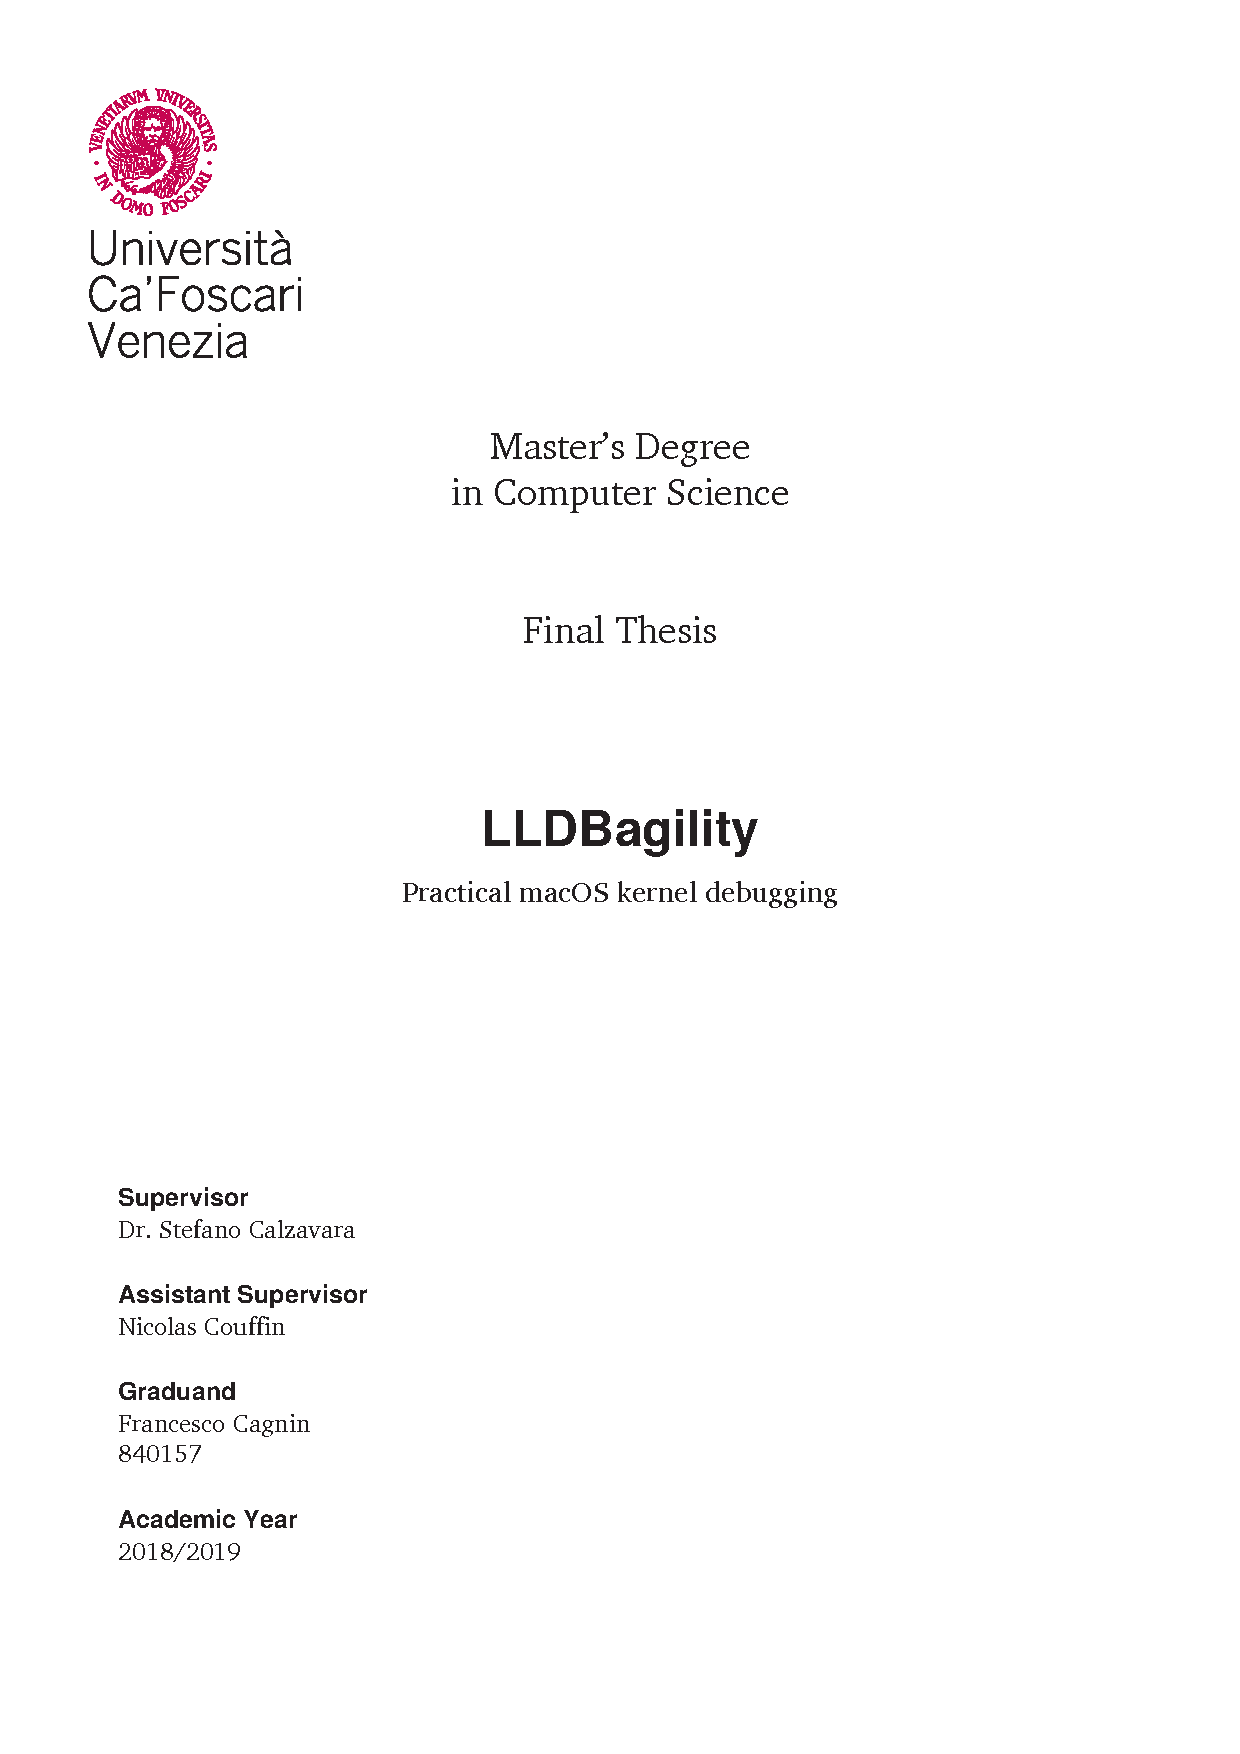
\includepdf{content/fsp.pdf}
\chapter{Acknowledgements}
This work concludes a long and at times difficult journey.

I express my deep gratitude to my supervisors, Nicolas Couffin, for his guidance and knowledge, and Stefano Calzavara, for his patience and valuable comments. My thanks extend to Quarkslab for a challenging internship in an office full of brilliant and pleasant colleagues.

To the old and new friends I met at Ca' Foscari, I am truly grateful for the many \enquote{intelligent} and meaningful conversations, countless moments of plain fun, and unforgettable days and nights of hacking (and pizza) with \emph{c00kies@venice}.

For their love, understanding, and financial support, I give my heartfelt thanks to my parents, Michele and Emilia.

\chapter{Abstract}
The effectiveness of debugging software issues largely depends on the capabilities of the tools available to aid in such task. At present, to debug the macOS kernel there are no alternatives other than the basic debugger integrated in the kernel itself or the GDB stub implemented in VMware Fusion. However, due to design constraints and implementation choices, both approaches have several drawbacks, such as the lack of hardware breakpoints and the capability of pausing the execution of the kernel from the debugger, or the inadequate performance of the GDB stub for some debugging tasks.

The aim of this work is to improve the overall debugging experience of the macOS kernel, and to this end LLDBagility has been developed. This tool enables kernel debugging via \glsentrylong{vmi}, allowing to connect the LLDB debugger to any unmodified macOS \glsentrylong{vm} running on a patched version of the VirtualBox hypervisor. This solution overcomes all the limitations of the other debugging methods, and also implements new useful features, such as saving and restoring the state of the \glsentrylong{vm} directly from the debugger. In addition, a technique for using the lldbmacros debug scripts while debugging kernel builds that lack debug information is provided. As a case study, the proposed solution is evaluated on a typical kernel debugging session.

\setcounter{tocdepth}{2}
\tableofcontents

\mainmatter
\blindmathtrue
\Blinddocument
% \chapter{Debugging the macOS kernel}\label{ch:dbgmacos}
This chapter describes how to debug recent version of the macOS kernel with a major focus on the the \glsentrylong{kdp}, \gls{xnu}'s mechanism for remote kernel debugging. Several sections are dedicated to explain how \gls{kdp} is implemented in the kernel, how to set up recent versions of macOS for remote debugging, and the notable limitations of this approach. The only valid alternative to \gls{kdp} is the GDB stub in VMware Fusion, presented at the end of the chapter, which brings improvements in many aspects but is also affected by a couple of different drawbacks. Unless otherwise stated, references to source code files are provided for \gls{xnu} 4903.221.2\footcite{XNU49032212} from macOS 10.14.1 Mojave, the most up-to-date source release available at the time of the study; at the time of writing, the sources of \gls{xnu} 4903.241.1\footcite{XNU49032411} from macOS 10.14.3 Mojave and \gls{xnu} 6153.11.26\footcite{XNU61531126} from macOS 10.15 Catalina have been published. Many of the outputs presented were edited or truncated for clarity of reading. As already noted in \cref{sec:xnudarwinmacos}, the terms \enquote{macOS}, \enquote{macOS kernel}, \enquote{Darwin kernel} and \enquote{\gls{xnu}} (this last referring exclusively to the specific build for macOS) will be used interchangeably, sacrificing a little accuracy for better readability.

\section{The \glsentrylong{kdp}}\label{sec:remotekdbg}
Like every other major \glsentrylong{os}\footcites[Windows supports remote kernel debugging with KDNET and the WinDbg debugger, and the Linux kernel with KGDB and the GDB debugger. See][]{WindowsDbg,LinuxDbg}, macOS supports remote kernel debugging to allow, under certain circumstances, a kernel-mode debugger running on a second machine to inspect and manipulate the state of the entire system. As mentioned in the kernel's README\footxnulink{README.md}{}{}, for such purpose \gls{xnu} implements the \glsentrylong{kdp}, a debugging interface to be interacted via a custom client--server protocol over \gls{udp}. As a typical kernel debugging mechanism, the \gls{kdp} solution consists of two parts:
\begin{itemize}
    \item A debug server running internally to the macOS kernel, listening for connections on port 41139, capable to alter the normal execution of the \glsentrylong{os} in order to execute debugging commands sent by a client. Throughout this work, this component is also referred to as the \gls{kdp} stub or agent.
    \item An external kernel-mode debugger running on a different machine, typically LLDB (see \cref{sec:lldb}), which manages the debugging session by sending requests to the \gls{kdp} server and eventually receiving back results and notifications of \gls{cpu} exceptions.
\end{itemize}

\gls{kdp} can be used either via Ethernet, FireWire or the serial interface, with the possibility of using Thunderbolt adapters in case such ports are not available; but since network interfaces can be used for debugging only when their driver explicitly supports \gls{kdp}, debugging over Wi-Fi is not supported\footcite{singh2006mac}. When the serial interface is used, \enquote{\gls{kdp} still encapsulates every message inside a fake Ethernet and \gls{udp} packet.}\footcite{miller2012ios} Since debugging has to be available as early as possible in the boot process, \gls{kdp} \enquote{does not use the kernel's networking stack but has its own minimal \gls{udp}/\gls{ip} implementation}\footcite{singh2006mac}.

The behaviour of the \gls{kdp} stub can be configured through \gls{bootarg} variables. The most important one is \lstinline{debug}, used to specify if and when the agent should activate, among other purposes; see \cref{lst:kdpdebugvalues} for a list of supported bitmasks. A summary scan of \gls{xnu} sources reveals further options: \lstinline{kdp_crashdump_pkt_size}, to set the size of the crash dump packet; \lstinline{kdp_ip_addr}, to set a static \gls{ip} address for the \gls{kdp} server; \lstinline{kdp_match_name}, to select which port to use (e.g.\ \lstinline{en1}) for Ethernet, Thunderbolt or serial debugging. Additionally, the IONetworkingFamily \glsentrylong{kext}\footcite{IONetworkingFamily} parses the variable \lstinline{kdp_match_mac} to match against a specific \gls{mac} address; this indicates that likely more \gls{kdp}-related options exist for configuring other \glsentrylongpl{kext}.

\lstinputlisting[style=block,linerange={419-447},firstnumber=419,caption={Bitmasks for the \lstinline{debug} \gls{bootarg} from \protect\xnulink{osfmk/kern/debug.h}{}{}},label={lst:kdpdebugvalues}]{darwin-xnu-xnu-4903.221.2/osfmk/kern/debug.h}

The current revision of the communication protocol used by \gls{kdp} is the 12th\footxnulink{osfmk/kdp/kdp.c}{109}{}, around since \gls{xnu} 1456.12.6\footcite{XNU1456126} from macOS 10.6 Snow Leopard. As in many other networking protocols, \gls{kdp} packets are composed of a common header and specialised bodies. The header, shown in \cref{lst:kdphdr}, contains, among other fields:
\begin{itemize}
    \item The type of \gls{kdp} request, such as \lstinline{KDP_READMEM64} or \lstinline{KDP_BREAKPOINT_SET}; the full set of possible requests is shown in \cref{lst:kdprequests}.
    \item A flag for distinguishing between requests and replies. With the exclusion of \lstinline{KDP_EXCEPTION} which is a notification\footxnulink{osfmk/kdp/kdp_protocol.h}{104}{}, \gls{kdp} requests are only sent by the debugger to the debuggee (and not vice versa)\footxnulink{osfmk/kdp/kdp_udp.c}{1087}{}.
    \item A sequence number to discard duplicate or out-of-order messages and retransmit replies\footxnulink{osfmk/kdp/kdp_udp.c}{1095}{}.
\end{itemize}
\lstinputlisting[style=block,linerange={167-173},firstnumber=167,caption={The \gls{kdp} packet header from \protect\xnulink{osfmk/kdp/kdp_protocol.h}{}{}},label={lst:kdphdr}]{darwin-xnu-xnu-4903.221.2/osfmk/kdp/kdp_protocol.h}

Instead, bodies contain each different fields that define all the possible \gls{kdp} requests and replies, as shown in \cref{lst:kdpreadmem64} as an example for \lstinline{KDP_READMEM64} packets.
\lstinputlisting[style=block,linerange={323-333},firstnumber=323,caption={The \lstinline{KDP_READMEM64} request and reply packets, as defined in \protect\xnulink{osfmk/kdp/kdp_protocol.h}{}{}},label={lst:kdpreadmem64}]{darwin-xnu-xnu-4903.221.2/osfmk/kdp/kdp_protocol.h}

As might be expected, \gls{xnu} assumes at most one \gls{kdp} client is attached to it at any given time. With the initial \lstinline{KDP_CONNECT} request, the debugger informs the kernel on which \gls{udp} port should notifications be sent back when exceptions occur. The interactions between the \gls{kdp} stub and the LLDB debugger during the attach phase are explored in detail in \Cref{ap:xnulldbcomm}.

\begin{figure}
    \centering
    \caption{Representation of a \lstinline{KDP_CONNECT} request packet. The \gls{kdp} header occupies the first 8 bytes, in which \lstinline{is_reply} is the eighth least significant bit. The \lstinline{req_reply_port} and \lstinline{exc_note_port} fields are the client \gls{udp} ports where to send replies and exception notifications. The \lstinline{greeting} field is an arbitrary null-terminated string of variable length.}\label{fig:kdpconnect}
    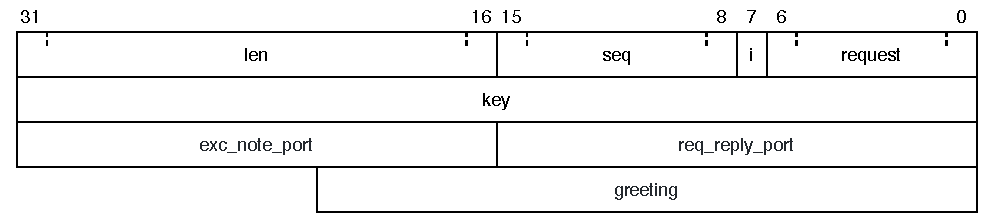
\includegraphics[width=\textwidth]{figures/kdpconnect.pdf}
\end{figure}

\subsection{Triggering the debugging stub}\label{sec:kdptriggers}
Naturally, the macOS kernel is not open to debugging by default. From a thorough search of \gls{xnu} sources and some testing, it seems the \gls{kdp} stub is allowed to take over the normal execution of the kernel only in three specific situations:
\begin{itemize}
    \item The kernel is a DEVELOPMENT or DEBUG build (see \cref{sec:kdk}) and the \lstinline{DB_HALT} bit has been set for the \lstinline{debug} \gls{bootarg}. If these conditions are met during kernel boot, then the debugging stub pauses the startup process waiting for a debugger.
    \lstinputlisting[style=block,linerange={273-283},firstnumber=273,caption={Checking for \lstinline{DB_HALT} in \protect\xnulink{osfmk/kern/debug.c}{}{}}]{darwin-xnu-xnu-4903.221.2/osfmk/kern/debug.c}

    \item The kernel is being run on a hypervisor (according to the \gls{cpu} feature flags outputted by the \lstinline{CPUID} instruction\footxnulink{osfmk/i386/machine_routines.c}{711}{}), the \lstinline{DB_NMI} bit has been set for the \lstinline{debug} \gls{bootarg} and a \gls{nmi} is triggered at any time during the \gls{os} execution.
    \lstinputlisting[style=block,linerange={626-643},firstnumber=626,caption={Starting \gls{kdp} on \glspl{nmi} in \protect\xnulink{osfmk/kdp/kdp_protocol.h}{}{}}]{darwin-xnu-xnu-4903.221.2/osfmk/i386/mp.c}
    % Works in VM with RELEASE
    % Does not seem to work in PM with RELEASE

    \item The \lstinline{debug} \gls{bootarg} has been set to any nonempty value (even invalid ones) and a panic occurs\footxnulink{osfmk/kern/debug.c}{290}{}, in which case the machine is not automatically restarted. Panics can be triggered programmatically with \gls{dtrace} from the command-line by executing \lstinline|dtrace -w -n "BEGIN{ panic(); }"| (assuming \gls{sip} is disabled, see \cref{sec:sip}).
    % Works in VM with RELEASE and debug=LOL
    % Does not work in VM with RELEASE and debug is not set (the machine restarts)
    % Does not seem to work in VM with RELEASE and debug set to empty string
\end{itemize}
Once the \gls{kdp} stub is triggered with any of these methods, the kernel simply loops waiting for an external debugger to attach. Notably, all three cases require changing the kernel \glspl{bootarg} to set the value of \lstinline{debug}.


\section{The \glsentrylong{kdk}}\label{sec:kdk}
For some macOS releases and \gls{xnu} builds, Apple publishes the corresponding \gls{kdk}, an accessory package for kernel debugging containing:
\begin{itemize}
    \item The DEVELOPMENT and DEBUG builds of the kernel, compiled with additional assertions and error checking with respect to the RELEASE version distributed with macOS; occasionally, also a KASAN build compiled with address sanitisation is included. Unlike RELEASE, these debug builds also contain full symbolic information.
    \item \gls{dwarf} companion files generated at compile time containing full debugging information, such as symbols and data type definitions, for each of the kernel builds included in the debug kit and also for some \glsentrylongpl{kext} shipped with macOS. If \gls{xnu} sources are also available, then source-level kernel debugging becomes possible (e.g.\ with LLDB and the command \lstinline{settings set target.source-map}\footcite{MacOSDebug9}).
    \item lldbmacros (discussed in \cref{sec:lldbmacros}), a set of debug scripts to assist the debugging of Darwin kernels.
\end{itemize}

All available \glspl{kdk} can be downloaded from the Apple Developer website\footcite{AppleKDK} after authenticating with a free Apple ID account. Being distributed as .pkg packages, \glspl{kdk} are usually installed through the macOS \gls{gui}, procedure that simply copies the package content into the local file system at \path{/Library/Developer/KDKs/}.

\begin{lstlisting}[style=out,language=bash,caption={Kernels builds from the \gls{kdk} for macOS 10.14.5 Mojave build 18F132}]
$ ls -l /Library/Developer/KDKs/KDK_10.14.5_18F132.kdk/System/Library/Kernels/
total 193192
-rwxr-xr-x  1 root  wheel  15869792 Apr 26  2019 kernel
drwxr-xr-x  3 root  wheel        96 Apr 26  2019 kernel.dSYM
-rwxr-xr-x  1 root  wheel  21428616 Apr 26  2019 kernel.debug
drwxr-xr-x  3 root  wheel        96 Apr 26  2019 kernel.debug.dSYM
-rwxr-xr-x  1 root  wheel  17018112 Apr 26  2019 kernel.development
drwxr-xr-x  3 root  wheel        96 Apr 26  2019 kernel.development.dSYM
-rwxr-xr-x  1 root  wheel  44591632 Apr 26  2019 kernel.kasan
\end{lstlisting}

\glsentrylongpl{kdk} are incredibly valuable for kernel debugging: information about data types makes it easy to explore kernel data structures through the debugger, and lldbmacros provide deep introspection capabilities. Unfortunately, for unknown reasons Apple does not distribute \glspl{kdk} for all macOS releases and updates, and when it does these packages are often published with weeks or months of delay. By searching the Apple Developer portal for the non-beta builds of macOS 10.14 Mojave as an example, at the time of this study in late May 2019 the \glspl{kdk} published on the same day as the respective macOS release were only three (18A391, 18C54 and 18E226) out of a total ten; one \gls{kdk} was released two weeks late (18B75); and no \gls{kdk} was provided for the other six kernel builds (18B2107, 18B3094, 18D42, 18D43, 18D109, 18E227). As of September 2019 four more macOS updates have been distributed, for which two \glspl{kdk} (18F132, 18G84) were promptly released and the other two (18G87 and 18G95) are missing. From a post on the Apple Developer Forums it appears that nowadays \enquote{the correct way to request a new \gls{kdk} is to file a bug asking for it.}\footcite{DevForums1}

\subsection{lldbmacros}\label{sec:lldbmacros}
As a replacement for the now abandoned kgmacros for GDB, since \gls{xnu} 2050.7.9\footcite{XNU205079} from macOS 10.8 Mountain Lion Apple has been releasing lldbmacros, a set of Python scripts for extending LLDB's capabilities with helpful commands and macros for debugging Darwin kernels. Examples are \lstinline{allproc}\footxnulink{tools/lldbmacros/process.py}{109}{} to display information about processes, \lstinline{pmap_walk}\footxnulink{tools/lldbmacros/pmap.py}{895}{} to perform virtual to physical address translation, and \lstinline{showallkmods}\footxnulink{tools/lldbmacros/memory.py}{1388}{} for a summary of all loaded \glspl{kext}.
\begin{lstlisting}[style=lldbsession,caption={Example output of the \lstinline{allproc} macro, executed during the startup process of macOS 10.14.5 Mojave build 18F132},label={lst:allproc}]
(lldb) allproc
Process 0xffffff800c8577f0
    name kextcache
    pid:11     task:0xffffff800c023bf8   p_stat:2      parent pid: 1
Cred: euid 0 ruid 0 svuid 0
Flags: 0x4004
    0x00000004 - process is 64 bit
    0x00004000 - process has called exec
State: Run
Process 0xffffff800c857c60
    name launchd
    pid:1      task:0xffffff800c022a70   p_stat:2      parent pid: 0
Cred: euid 0 ruid 0 svuid 0
Flags: 0x4004
    0x00000004 - process is 64 bit
    0x00004000 - process has called exec
State: Run
Process 0xffffff8006076b58
    name kernel_task
    pid:0      task:0xffffff800c023048   p_stat:2      parent pid: 0
Cred: euid 0 ruid 0 svuid 0
Flags: 0x204
    0x00000004 - process is 64 bit
    0x00000200 - system process: no signals, stats, or swap
State: Run
\end{lstlisting}

If the \gls{kdk} for the kernel being debugged is installed in the host machine, just after attaching LLDB will detect the availability of lldbmacros and suggest loading them with the command \lstinline{command script import}. In addition to be distributed as part of any \glspl{kdk}, lldbmacros are also released together with \gls{xnu} sources; however, to operate properly (or at all) most macros require debugging information, which is released only within the debug kits in the form of \gls{dwarf} companion files.


\section{Setting macOS up for remote debugging}\label{sec:setup}
Apple's documentation on kernel debugging\footcite{DarwinDoc1} is outdated (ca. 6 years old as of 2019) and no longer being updated, but fortunately the procedure described there has not changed much to this day. In addition, many third-party guides on how to set up recent versions of macOS for debugging are available on the Internet\footcites{MacOSDebug2,MacOSDebug3,MacOSDebug4,MacOSDebug5}. According to all these resources, the suggested steps for enabling remote kernel debugging via \gls{kdp} on a modern macOS target machine involve:
\begin{enumerate}
    \item Finding the exact build version of the macOS kernel to debug, for example by executing the \path{sw_vers} command-line utility and reading its output at the line starting with \lstinline{BuildVersion}.
\begin{lstlisting}[style=out,language=bash,caption={Example output of the \protect\path{/usr/bin/sw_vers} utility}]
$ sw_vers
ProductName:	Mac OS X
ProductVersion:	10.15.2
BuildVersion:	19C57
\end{lstlisting}

    \item Downloading and installing the \glsentrylong{kdk} for the specific build version, so to obtain a copy of the debug builds of the kernel. The same \gls{kdk} should be installed also in the host machine (supposing it's running macOS), so to give LLDB or any other debugger access to a copy of the kernel executables that is going to be debugged.

    \item Disabling \glsentrylong{sip} from macOS Recovery, to remove the restrictions on replacing the default kernel binary and modifying \glspl{bootarg} in \gls{nvram}.

    \item Installing at least one of the debug builds of the kernel by copying the desired executable (e.g.\ \lstinline{kernel.development}) from the directory of the installed \gls{kdk} to \path{/System/Library/Kernels/}.

    \item Setting the \lstinline{kcsuffix} and \lstinline{debug} \glspl{bootarg} to appropriate values, the first to select which of the installed kernel builds to use for the next macOS boot and the second to actually enable the debugging features of the kernel. \Glspl{bootarg} can be set using the \lstinline{nvram} command-line utility, as shown in \cref{lst:nvram}. Proper values for \lstinline{kcsuffix} are typically \enquote{development}, \enquote{debug} or \enquote{kasan}; valid bitmasks for \lstinline{debug} were listed in \cref{lst:kdpdebugvalues}. Apple's docs and other resources\footcite{DarwinDoc1,MacOSDebug10} also mention setting \lstinline{pmuflags=1} to avoid watchdog timer problems, but this parameter doesn't seem to be parsed anywhere in recent \gls{xnu} sources (although it could still be used by some \glsentrylong{kext}); possibly related, the READMEs of some recent \glspl{kdk} suggest instead to set \lstinline{watchdog=0} to \enquote{prevent the macOS watchdog from firing when returning from the kernel debugger.}

\begin{lstlisting}[style=out,language=bash,caption={Example usage of the \protect\path{/usr/sbin/nvram} utility},label={lst:nvram}]
$ sudo nvram boot-args="-v kcsuffix=development debug=0x4"
$ nvram -p | grep boot-args
boot-args	-v kcsuffix=development debug=0x4
\end{lstlisting}

    \item Recreating the \enquote{kextcache}, to allow macOS to boot with a different kernel build than the last one used. Caches can apparently be rebuilt either by executing the command \lstinline{touch} on the \lstinline{/System/Library/Extensions/} directory of the installation target volume, as recommended by the \path{kextcache} manual page\footcite{BSDkextcache}, or by executing the command \lstinline{kextcache -invalidate /Volumes/<Target Volume>}, as suggested by several other resources including the READMEs of some \glspl{kdk}. Both methods appear to work, even though it's not clear which of the two is to be preferred on recent versions of macOS.

    \item Lastly, rebooting the machine into macOS and triggering the activation of the debugging stub in the kernel, in accordance with how it has been set up via the \lstinline{debug} \gls{bootarg}. In all cases, either during boot or in response to panics or \glspl{nmi}, the kernel will deviate from its normal execution to wait for a remote debugger to connect; at that point, any debugger supporting \gls{kdp} (such as LLDB with the \lstinline{kdp-remote} command) can attach to the kernel and start debugging.
\end{enumerate}

Although these instructions allow to correctly set up a Mac for kernel debugging, they are in some parts neither exhaustive nor completely accurate. Some observations:
\begin{itemize}
\item All resources cited above suggest to disable \gls{sip}, but this is not required at all: installing the debug binaries and setting \glspl{bootarg} can be done directly from macOS Recovery without disabling \gls{sip} for macOS (operation that requires a reboot into macOS Recovery anyway).

\item Similarly, no resource points out that to work properly \gls{kdp} doesn't actually require \gls{sip} to be turned off, and so that it's always possible to re-enable it prior to debugging: depending on the parts of the kernel that will be analysed, it may be desirable to leave this security mechanism on.

\item Mentioned only once and superficially, installing a debug build of the kernel is not strictly required since it is also possible to debug the RELEASE kernel (see \cref{sec:kdptriggers}), although it's generally preferable as debug executables aid the debugging process in multiple ways (e.g.\ with address sanitisation).
\end{itemize}

To eventually restore macOS to the RELEASE kernel, it is at minimum required to:
\begin{itemize}
\item Remove the \lstinline{kcsuffix} argument from the \glspl{bootarg}.
\item Remove all kernel caches at \path{/System/Library/Caches/com.apple.kext.caches/Startup/kernelcache.*}. and all prelinked kernels at \path{/System/Library/PrelinkedKernels/prelinkedkernel.*}.
\end{itemize}

Instead of using a physical Mac, as shown in some other online tutorials\footcites{MacOSDebug6,MacOSDebug7,MacOSDebug8,MacOSDebug10} it is also possible to debug macOS when this is running on a \glsentrylong{vm}, without changes in the configuring procedure described above; this is very convenient since \glspl{vm} are much easier to set up, debug, reuse and dispose than physical machines. The process is illustrated in \cref{fig:vmdbg}. As additional benefit, when the target machine is a \gls{vm} rebooting into macOS Recovery to modify \gls{nvram} and \glspl{bootarg} is not required, since this operation is usually done by the hypervisor bypassing the guest \gls{os} (e.g. with the VirtualBox command \lstinline{VBoxManage setextradata "<Vm Name>" "VBoxInternal2/EfiBootArgs" "<Var>=<Value>"}). Regardless of how the \glsentrylong{vm} running macOS is used, to comply with the Apple \gls{eula} the general consensus\footcite{CommunityForums1} is that it must run on top of another copy of macOS installed directly on Apple hardware, i.e.\ a real Mac.

\begin{figure}
    \centering
    \caption{Debugging macOS running on a \glsentrylong{vm} with \gls{kdp}}\label{fig:vmdbg}
    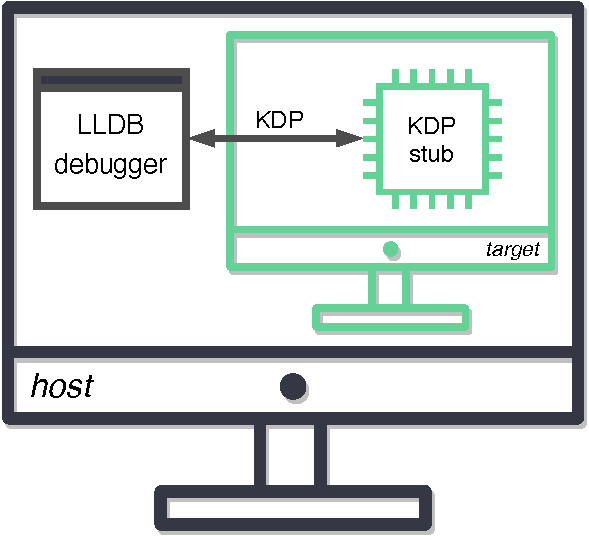
\includegraphics[width=70mm]{figures/debugging-vm-debugging.pdf}
\end{figure}


\section{An example debugging session}\label{sec:dbgsession}
This section demonstrates a simple \gls{kdp} debugging session, conducted on a host machine running macOS 10.15 Catalina build 19A602 with LLDB 1100.0.28.19 and a target VirtualBox \gls{vm} running macOS 10.14.5 Mojave build 18F132. Both machines installed the \glsentrylong{kdk} build 18F132. The target machine was configured as explained in \cref{sec:setup}: first, \gls{sip} was fully disabled from macOS Recovery by executing the command \lstinline{csrutil disable} in the Terminal application; then, the DEBUG kernel was copied from \path{/Library/Developer/KDKs/KDK_10.14.5_18F132.kdk/System/Library/Kernels/kernel.debug} to \path{/System/Library/Kernels/}; next, the \gls{bootarg} variable was set to \lstinline{"kcsuffix=debug debug=0x1"}; lastly, the \gls{kext} cache was rebuilt in consequence of executing the command \lstinline{touch /System/Library/Extensions/}.

Since \lstinline{DB_HALT} was set, shortly after initiating booting on the target machine the \gls{kdp} stub assumed control and eventually the string \enquote{Waiting for remote debugger connection.} was printed on screen; LLDB, running on the host machine, could then attach with the \lstinline{kdp-remote} command:
\begin{lstlisting}[style=lldbsession,label={lst:kdpremote}]
(lldb) kdp-remote 10.0.2.15
Version: Darwin Kernel Version 18.6.0: Thu Apr 25 23:15:12 PDT 2019; root:xnu_debug-4903.261.4~1/DEBUG_X86_64; UUID=4578745F-1A1F-37CA-B786-C01C033D4C22; stext=0xffffff800f000000
Kernel UUID: 4578745F-1A1F-37CA-B786-C01C033D4C22
Load Address: 0xffffff800f000000
warning: 'kernel' contains a debug script. To run this script in this debug session:

    command script import "/System/. . ./KDKs/KDK_10.14.5_18F132.kdk/. . ./kernel.py"

To run all discovered debug scripts in this session:

    settings set target.load-script-from-symbol-file true

Kernel slid 0xee00000 in memory.
Loaded kernel file /System/. . ./KDKs/KDK_10.14.5_18F132.kdk/System/Library/Kernels/kernel.debug
Loading 68 kext modules ----.--.------.---....--------------.---------------......-------.-- done.
Failed to load 53 of 68 kexts:
    com.apple.AppleFSCompression.AppleFSCompressionTypeDataless 38BD7794-FDCB-3372-8727-B1209351EF47
    com.apple.AppleFSCompression.AppleFSCompressionTypeZlib     8C036AB1-8BF0-32BE-9B7F-75AD4C571D34
    . . .
    com.apple.security.quarantine                               11DE02EC-241D-35AA-BBBB-A2E7969F20A2
    com.apple.security.sandbox                                  ECE8D480-5444-3317-9844-559B22736E5A
Process 1 stopped
* thread #1, stop reason = signal SIGSTOP
    frame #0: 0xffffff800f2e3bf5 kernel.debug`kdp_call at kdp_machdep.c:331:1
Target 0: (kernel.debug) stopped.
\end{lstlisting}

The debugger had now control of the target machine. Active stack frames were retrieved with the \lstinline{bt} command:
\begin{lstlisting}[style=lldbsession]
(lldb) bt
* thread #1, stop reason = signal SIGSTOP
    * frame #0: 0xffffff800f2e3bf5 kernel.debug`kdp_call . . .
    frame #1: 0xffffff800f05e28f kernel.debug`kdp_register_send_receive . . .
    frame #2: 0xffffff7f901b82df IONetworkingFamily`IOKernelDebugger::registerHandler . . .
    frame #3: 0xffffff7f901b8429 IONetworkingFamily`IOKernelDebugger::handleOpen . . .
    frame #4: 0xffffff800fb94be5 kernel.debug`IOService::open . . .
    frame #5: 0xffffff7f901b7910 IONetworkingFamily`IOKDP::start . . .
    frame #6: 0xffffff800fb96ac2 kernel.debug`IOService::startCandidate . . .
    frame #7: 0xffffff800fb960eb kernel.debug`IOService::probeCandidates . . .
    frame #8: 0xffffff800fb8e351 kernel.debug`IOService::doServiceMatch . . .
    frame #9: 0xffffff800fb97626 kernel.debug`_IOConfigThread::main . . .
    frame #10: 0xffffff800f2c278e kernel.debug`call_continuation + 46
\end{lstlisting}

\gls{cpu} registers could be read and modified:
\begin{lstlisting}[style=lldbsession]
(lldb) register read
General Purpose Registers:
        rax = 0xffffff800fec5930  kernel.debug`halt_in_debugger
        rbx = 0xffffff801c8830c0
        rcx = 0x0000000000000001
        rdx = 0xffffff801241104c
        rdi = 0x0000000000000000
        rsi = 0xffffff800fc726cd  "_panicd_corename"
        rbp = 0xffffff81952e5b00
        rsp = 0xffffff81952e5b00
        r8 = 0xffffff81952e5ad0
        r9 = 0x0000000000000000
        r10 = 0x837bdd93184000bc
        r11 = 0x0000000000000079
        r12 = 0xffffff7f901bbd78  IONetworkingFamily`IONetworkController::debugRxHandler(IOService*, void*, unsigned int*, unsigned int) at IONetworkController.cpp:1594
        r13 = 0xffffff7f901bbd98  IONetworkingFamily`IONetworkController::debugSetModeHandler(IOService*, bool) at IONetworkController.cpp:1635
        r14 = 0xffffff801bcde530
        r15 = 0xffffff7f901d06d8  IONetworkingFamily`IONetworkInterface::gMetaClass
        rip = 0xffffff800f2e3bf5  kernel.debug`kdp_call + 5 at kdp_machdep.c:331:1
    rflags = 0x0000000000000202
        cs = 0x0000000000000008
        fs = 0x0000000000000000
        gs = 0x0000000000000000
(lldb) register write $rax 0xffffffff
(lldb) register read $rax
        rax = 0x00000000ffffffff
\end{lstlisting}

Memory could also be read and modified:
\begin{lstlisting}[style=lldbsession]
(lldb) memory write -s4 $rsi 41414141
(lldb) memory read $rsi
0xffffff800fc726cd: 41 41 41 41 69 63 64 5f 63 6f 72 65 6e 61 6d 65  AAAAicd_corename
0xffffff800fc726dd: 00 6b 64 70 5f 69 70 5f 61 64 64 72 00 5f 6b 64  .kdp_ip_addr._kd
\end{lstlisting}

A breakpoint was installed on the \lstinline{unix_syscall64()} routine:
\begin{lstlisting}[style=lldbsession]
(lldb) breakpoint set -a unix_syscall64
Breakpoint 1: where = kernel.debug`unix_syscall64 at systemcalls.c:275, address = 0xffffff800fae9210
\end{lstlisting}

Then, execution was resumed:
\begin{lstlisting}[style=lldbsession]
(lldb) continue
Process 1 resuming
\end{lstlisting}

And shortly thereafter the breakpoint fired, causing the kernel to stop its regular execution and return the control to LLDB:
\begin{lstlisting}[style=lldbsession]
Process 1 stopped
* thread #1, stop reason = breakpoint 1.1
    frame #0: 0xffffff800fae9210 kernel.debug`unix_syscall64(state=<unavailable>) at systemcalls.c:275
Target 0: (kernel.debug) stopped.
\end{lstlisting}

The debugging session was then terminated.


\section{Limitations}\label{sec:kdplimitations}
As discussed and demonstrated in the previous sections, the \glsentrylong{kdp} offers most of the basic kernel debugging capabilities, such as reading and modifying \gls{cpu} registers and memory and pausing the execution of the system with breakpoints. However, due to design and implementation choices this solution also presents several limitations and inconveniences, listed below in no particular order:
\begin{itemize}
    \item To enable \gls{kdp} and the debugging capabilities of the kernel it is required at minimum to set the \lstinline{debug} \gls{bootarg} in \gls{nvram} (see \cref{sec:kdptriggers}), but this modification requires in turn to at least reboot into macOS Recovery, either to update the \glspl{bootarg} directly or to disable \gls{sip}. As already mentioned, this isn't necessary when the machine is a \gls{vm}.

    \item Debugging the initial part of the kernel boot process is not possible since debugging can start only after the initialisation of the \gls{kdp} stub, which happens relatively late in the startup phase.

    \item The debugging process alters in possibly unknown ways the default behaviour of the kernel and of some \glsentrylongpl{kext} included in macOS; debugging a system not operating on default settings may not be desirable, especially in some security research contexts.

    \item Debugging has various side effects on the whole system, including: the modification of the value of global variables (e.g.\ \lstinline{kdp_flag}\footxnulink{osfmk/kdp/kdp_udp.c}{252}{433}); the mapping of the \enquote{low global vector} page at a fixed memory location\footxnulink{osfmk/x86_64/pmap.c}{1171}{}; and the altering of kernel code due to the temporary replacement of instructions with the \lstinline{0xCC} opcode for software breakpoints. All these and likely others may impede debugging in adversarial situations, in which malware or exploits actively try to detect if the system is being debugged in order to conceal their behaviour; for these programs it is then sufficient to examine \gls{nvram} or other global variables, or to detect breakpoints by searching code sections for \lstinline{0xCC} bytes.

    \item Hardware breakpoints and watchpoints are not supported. LLDB sets breakpoints by issuing \lstinline{KDP_BREAKPOINT_SET} or \lstinline{KDP_BREAKPOINT_SET64} requests which trigger the execution of \lstinline{kdp_set_breakpoint_internal()}\footxnulink{osfmk/kdp/kdp.c}{900}{}, whose implementation makes clear that only software breakpoints are used. The unavailability of hardware breakpoints is corroborated by the facts that there is no \gls{kdp} request in kernel sources to do so and that the \lstinline{KDP_WRITEREGS} request doesn't allow to modify \gls{x86} debug registers\footxnulink{osfmk/kdp/ml/x86_64/kdp_machdep.c}{240}{}. Moreover, the lack of watchpoints is also explicitly stated in LLDB sources\footlldblink{source/Plugins/Process/MacOSX-Kernel/ProcessKDP.cpp}{699}{}.

\begin{lstlisting}[style=lldbsession,caption={Trying to set watchpoints in a \gls{kdp} debugging} session]
(lldb) watchpoint set expression &((boot_args *)PE_state.bootArgs)->CommandLine
error: Watchpoint creation failed (addr=0xffffff8012411008, size=8).
error: watchpoints are not supported in kdp remote debugging
\end{lstlisting}

    \item Rather strangely, LLDB cannot pause the execution of the kernel once this has been resumed\footcite{MacOSDebug7} (e.g.\ with the \lstinline{continue} command). Inspection of \gls{xnu} sources suggests that this feature seems to be supported by \gls{kdp} with the \lstinline{KDP_SUSPEND} request, although this has not been tested. At present, the only known way to pause a running macOS and return the control to the debugger is to trigger a breakpoint trap manually, for example with \gls{dtrace} from the command-line of the debuggee by executing \lstinline|dtrace -w -n "BEGIN{ breakpoint(); }"|, or by generating an \gls{nmi}, either with specific hardware keys combinations if the target machine is a real Mac (e.g.\ by holding down both the left and right command keys while pressing the power button\footcite{DarwinDoc9}) or through hypervisor commands in the case of \glsentrylongpl{vm} (e.g.\ the VirtualBox command \lstinline{VBoxManage debugvm "<Vm Name>" injectnmi}).
    % http://trineo.net/p/17/06_debug_xnu.html
    % Yet if you continue execution of the kernel, you can interrupt the kernel manually via Command-Option-Control-Shift-Escape key.

\begin{lstlisting}[style=lldbsession,caption={Trying to interrupt a \gls{kdp} debugging} session]
(lldb) process interrupt
error: Failed to halt process: Halt timed out. State = running
\end{lstlisting}

    \item After disconnecting from the remote kernel for any reason, it's apparently not always possible to reattach: \enquote{Do not detach from the remote kernel!}\footcite{DarwinDoc1}

    \item Multiple users report the whole debugging process via \gls{kdp} to be frail, especially when carried out over \gls{udp}: \enquote{LLDB frequently gets out of sync or loses contact with the debug server, and the kernel is left in a permanently halted state.}\footcite{MacOSDebug9} This phenomenon seems to be acknowledged even in \gls{xnu} sources\footxnulink{osfmk/kdp/kdp_udp.c}{1346}{}.
\end{itemize}

Lastly, a significant obstacle to the efficacy of the debugging process is the absence of lldbmacros for most macOS releases, being part of the \gls{kdk} which are released sporadically, as mentioned in \cref{sec:kdk}.


\section{Other debugging options}
Mentioned for completeness, at least two other methods for kernel debugging have been supported at some point in several \gls{xnu} releases: the DDB debugger and the kmem \gls{devicefile}. Unfortunately, these do not constitute neither an alternative nor a supplement to \gls{kdp} debugging, since DDB has been removed from kernel sources since a few releases and kmem only offers access to kernel memory (in addition to be somewhat deprecated). A third debugging option is the GDB stub implemented in VMware Fusion, which completely bypasses \gls{kdp} by moving the debugging process to the hypervisor level; this approach is explored further in the next chapter.

\subsection{DDB}\label{sec:kdbddb}
The archived Apple's documentation\footcite{DarwinDoc1} suggests to use the DDB debugger (or its predecessor, KDB), built entirely into the kernel and to be interacted with locally through a hardware serial line, when debugging remotely via \gls{kdp} is not possible or problematic, e.g.\ when analysing hardware interrupt handlers or before the network hardware is initialised. DDB first appeared as a facility of the Mach kernel (of which \gls{xnu} is a derivative\footcite{singh2006mac}) developed at Carnegie Mellon University in the nineties, and apparently can still be found in most descendants of the BSD \glsentrylong{os}\footcites{FreeBSDDDB,OpenBSDDDB,NetBSDDDB}. On macOS, enabling DDB required \enquote{building a custom kernel using the DEBUG configuration.}\footcite{DarwinDoc1} Support for this debugger seems however to have been dropped after \gls{xnu} 1699.26.8\footcite{XNU1699268}, given that the directory \path{osfmk/ddb/} containing all related files was removed in the next release; nevertheless, some references to DDB and KDB are still present in \gls{xnu} sources, such as the bitmask \lstinline{DB_KDB} for the \lstinline{debug} \gls{bootarg}\footxnulink{osfmk/kern/debug.h}{424}{}.

\subsection{kmem}\label{sec:kmem}
The README of the \glsentrylong{kdk} for macOS 10.7.3 Lion build 11D50, among others, alludes to the possibility of using the \gls{devicefile} \path{/dev/kmem} for limited self-debugging:
\blockquote{Live (single-machine) kernel debugging was introduced in Mac OS X Leopard. This allows limited introspection of the kernel on a currently-running system. This works using the normal kernel and the symbols in this \glsentrylong{kdk} by specifying \lstinline{kmem=1} in your \glspl{bootarg}; the DEBUG kernel is not required.}
This method still works in recent macOS releases provided that \glsentrylong{sip} is disabled, but newer \glspl{kdk} do not mention it anymore, and a note from Apple's docs\footcite{DarwinDoc3} says that support for kmem will be removed entirely in a unspecified future.

\subsection{GDB stub in VMware Fusion}\label{sec:stubvmfusion}
VMware Fusion is a type-2 hypervisor for Mac and macOS developed by VMware\footcite{VMware}. Among other features, this software implements and exposes a GDB remote stub, allowing any external debugger implementing the GDB \glsentrylong{rsp} (e.g.\ GDB itself or LLDB with the \lstinline{gdb-remote} command) to debug running \glsentrylongpl{vm} through \glsentrylong{vmi} (see \cref{sec:vmi}), no matter the guest \gls{os}. The process is represented in \cref{fig:fusiondbg}. In the case of macOS, VMware Fusion makes then possible debugging \gls{xnu} without relying on \gls{kdp}, eliminating many of the restrictions that it comports; for instance, the GDB stub has no problems with interrupting the execution of the kernel at any time. While being a very solid alternative to \gls{kdp}, this solution is not without its drawbacks:
\begin{itemize}
    \item VMware Fusion is not free.
    \item Using the GDB protocol, notoriously slow\footcite{Couffin2016Winbagility,sally2010pro,GDBSlow2,GDBSlow3} because of the high amount of data exchanged between GDB and its stub, makes debugging difficult when trying to analyse race conditions or when breakpoints are hit very frequently, in which case the machine is often slowed down to the point that debugging is impossible.
\end{itemize}

\begin{figure}
    \centering
    \caption{Debugging macOS running on a \glsentrylong{vm} with the GDB stub in VMware Fusion. The \gls{kdp} stub is not running, since debugging occurs at the hypervisor level.}\label{fig:fusiondbg}
    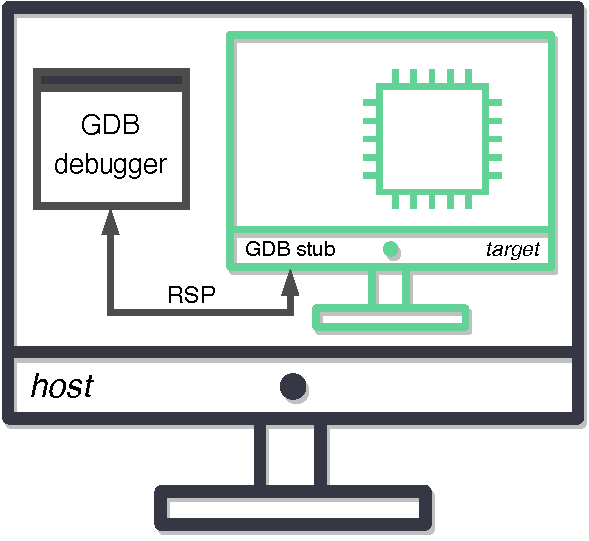
\includegraphics[width=70mm]{figures/debugging-fusion-debugging.pdf}
\end{figure}

Multiple guides exist on the Internet explaining how to set up VMware Fusion for macOS debugging\footcites{MacOSDebug9,MacOSDebug11,MacOSDebug12}.


% \appendix
% \include{content/a01}

\backmatter
\nocite{*}% for printing all resources from the bibliography including the ones not explicitly cited
\printnoidxglossaries
\printbibliography[type=online,heading=bibintoc,title={Online sources}]
\printbibliography[nottype=online,heading=bibintoc,title={Printed sources}]

\glsaddallunused
\end{document}
